%=== tech/fonctions/signes_10.tex || Fonctions || Signes

On considère une fonction $f$ définie sur $\R$ dont le tableau de signes est donné ci-dessous.

\smallskip

\hfill\begin{tikzpicture}
  \tkzTabInit{$x$/0.8,$f(x)$/0.8}{$-\infty$,$2$,$+\infty$}
    \tkzTabLine{,+,z,-,}
\end{tikzpicture}\hfill\null

\smallskip

Parmi les quatre expressions proposées pour la fonction $f$, une seule est possible.

\smallskip

\eamreponsesautom[2]{$f(x)=-3 x+6$}{$f(x)=x+2$}{$f(x)=x-2$}{$f(x)=-4 x+2$}